\section{Response Surface of the Discrepancy}
\label{sec:response}

As discussed earlier in Section~\ref{sec:intro}, bulk thermal conductivity estimates using NEMD simulations
are lower than measured values primarily due to reduction in mean free path associated with phonon transport. 
Additionally, the introduction of thermostats causes significant fluctuations in the applied temperature gradient,
especially in their vicinity. 
We illustrate this phenomenon by plotting the temperature 
distribution along the length of the bar in Figure~\ref{fig:kapitza}. 

\begin{figure}[htbp]
 \begin{center}
  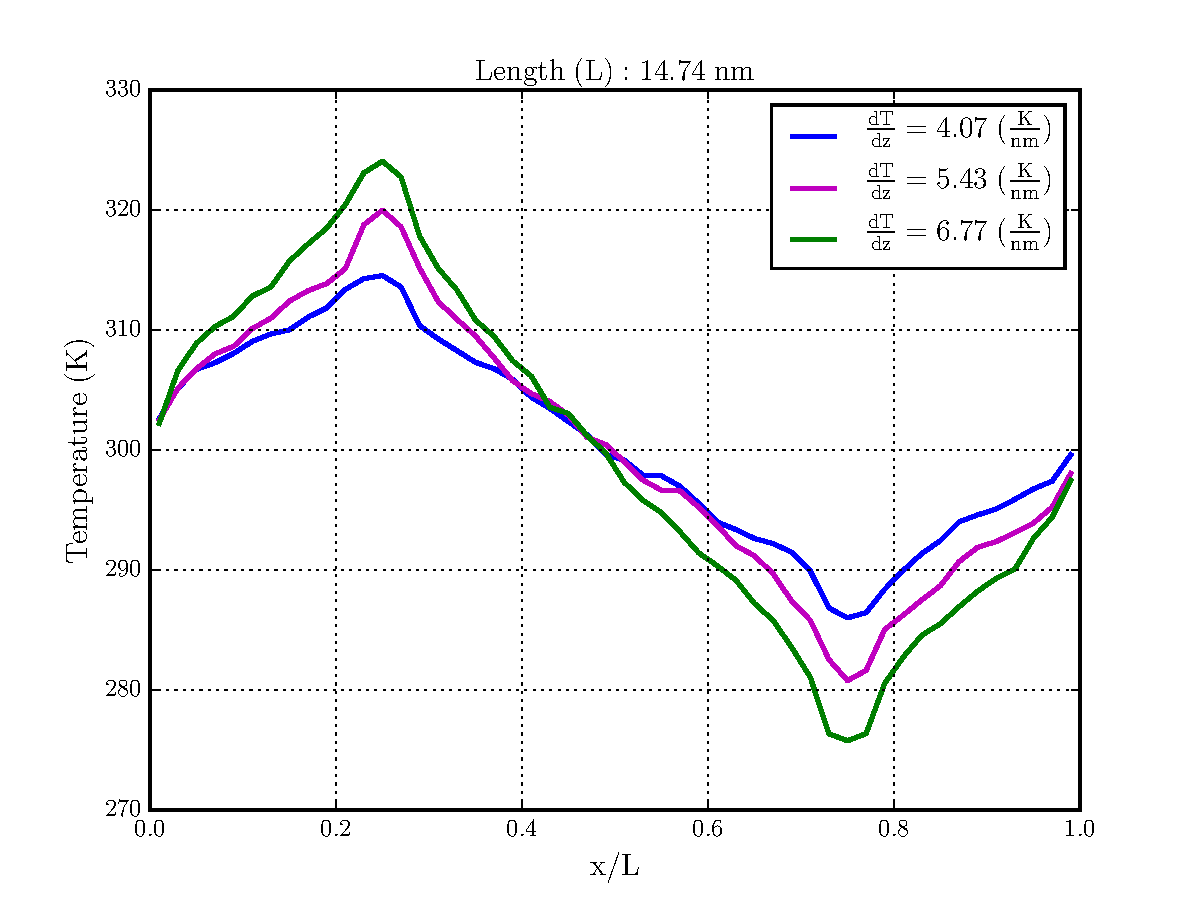
\includegraphics[width=0.70\textwidth]{temp_plot}
\caption{Temperature distribution along a Si bar of length 14.74~nm for
different scenarios of applied temperature gradient.}
\label{fig:kapitza}
\end{center}
\end{figure}

In this section, we focus on the impact of
system size, specifically the length of the Si bar as well as the applied temperature gradient on the discrepancy
in bulk thermal conductivity between NEMD predictions and experimental data. For this purpose, we consider
a range of values for the bar length and the temperature gradient. In order to determine the discrepancy trends, one
might consider evaluating the thermal conductivity using NEMD simulations for a large set of values of length and
temperature gradient. However, considering the computational expense associated with each pair of values, this approach quickly
becomes computationally prohibitive. Instead, we construct a response surface using a 2D 
PC representation of the discrepancy which requires NEMD predictions for a small number of
combinations of length and temperature gradient values as discussed in the following section. 

\subsection{Polynomial Chaos Response Surface}

The PC response surface approximates the functional relationship between independent
and uncertain 
inputs~$(\bm{\theta})$ to a model with the output $\mathcal{Y}$. Essentially, it is a truncated expansion with polynomial 
basis functions that converges in a least-squares sense. For an accurate PC representation, the output should
vary smoothly with respect to the uncertain inputs~\cite{Vohra:2014}  and must
be L-2 integrable:

\be
\mathbb{E}[\mathcal{Y}^2] = \int_{\mathcal{D}_{\bm{\theta}}} \mathcal{Y}^2 \mathbb{P}(\bm{\theta}) 
d\bm{\theta} < \infty
\ee

\noindent where $\mathcal{D}_{\bm{\theta}}$ is the domain of the input parameter space and 
$\mathbb{P}(\bm{\theta})$ is the joint probability distribution of individual components of $\bm{\theta}$.
In the present setting, $\bm{\theta}$:~$\{L,\frac{dT}{dz}\}$ and the output, $\mathcal{Y}$ is the
discrepancy~($\epsilon_{\mbox{\tiny{d}}}$ = 
$\lvert\kappa_{\mbox{\tiny{MD}}}$ - $\kappa_{\mbox{\tiny{E}}}\rvert$)
in bulk thermal conductivity predictions from 
NEMD~($\kappa_{\mbox{\tiny{MD}}}$) and experimental data~($\kappa_{\mbox{\tiny{E}}}$), at a 
given temperature, $T$. The PC representation of $\epsilon_{\mbox{\tiny{d}}}$ is given as:

\be
\epsilon_{\mbox{\tiny{d}}} \approx \mathcal{\epsilon}_{\mbox{\tiny{d}}}^{\mbox{\tiny{PCE}}} = 
\sum_{\bm{k}\in\mathcal{I}} c_{\bm{k}}(T)\Psi_{\bm{k}}(\bm{\xi(\theta)}) 
\ee

\noindent Individual components of the uncertain input vector, $\bm{\theta}$ are parameterized in terms of canonical random 
variables, $\bm{\xi}$ distributed uniformly in the interval $[-1,1]$. 
 $\Psi_{\bm{k}}$'s are multivariate polynomial basis functions, orthonormal with respect to the joint probability 
 distribution of $\bm{\xi}$. The degree of truncation in the above expansion is denoted by $\bm{k}$, a subset of
 the multi-index set $\mathcal{I}$ that comprises of individual degrees of univariate polynomials in $\Psi_{\bm{k}}$.
The PC coefficients, $c_{\bm{k}}$'s can be estimated using either numerical quadrature or advanced techniques
involving basis pursuit de-noising~\cite{Peng:2014}, compressive
sampling~\cite{Hampton:2015}, and least angle regression~\cite{Blatman:2011} suited for large-dimensional
applications. However, in our case, since the response surface is 2D, we use Gauss-Legendre quadrature to
obtain accurate estimates of the PC coefficients. 
\bigskip

In order to construct the response surface of the discrepancy, we consider respective intervals for the Si bar length,
$L$ and the applied temperature gradient, $\frac{dT}{dz}$ as $[50a,100a]$~($\angstrom$) and
 $[\frac{1.5}{a},\frac{2.5}{a}]$~($\frac{\mbox{\tiny{K}}}{\tiny{\angstrom}}$); $a$ being the lattice constant. For the considered length interval, the number of atoms in the
simulation were observed to range from 201344 to 379456. It must be noted that our 
focus is on illustrating a methodology for constructing a response surface that
sufficiently captures the relationship between the inputs: $L$, $\frac{dT}{dz}$ and
the discrepancy, $\epsilon_d$. Hence, we believe
that the considered range for $L$ is large enough to be able to capture the input-output
trends as presented further below, while ensuring reasonable computational effort.
Additionally, the underlying noise associated with NEMD simulations was found to be
negligible in the considered range for $\frac{dT}{dz}$ since we use average temperature
at the bin point during the data production NVE ensemble.
 
NEMD predictions of $\kappa_{\text{MD}}$
are obtained at 25 Gauss-Legendre quadrature nodes (or points) in the 2D parameter 
space as highlighted in Figure~\ref{fig:rs2}(a)~and~\ref{fig:rs2}(b). 
Note that 5 points are considered along $L$ and
$\frac{dT}{dz}$ assuming that a fourth order polynomial basis would be sufficient in
both cases, and the associated computational effort is not too large. 
Later, we assess the validity of our assumption by verifying the accuracy of the resulting
response surface.
 
 The discrepancy between $\kappa_{\mbox{\tiny{MD}}}$ and $\kappa_{\mbox{\tiny{E}}}$ is computed at the quadrature nodes as illustrated in Figure~\ref{fig:rs1}(a) to estimate the PC coefficients. The spectrum of 
 resulting PC coefficients is illustrated in Figure~\ref{fig:rs1}(b). 
Note that the value of $\kappa_{\mbox{\tiny{E}}}$ is considered to be 149~W/m/K as provided 
 in~\cite{Shanks:1963}. Response surfaces constructed at the bulk temperature, $T$ = 300~K and 500~K are 
 illustrated
 in Figure~\ref{fig:rs2}(a) and~\ref{fig:rs2}(b) respectively.

\begin{figure}[htbp]
\begin{center}
\begin{tabular}{cc}
  \hspace{-12mm}
  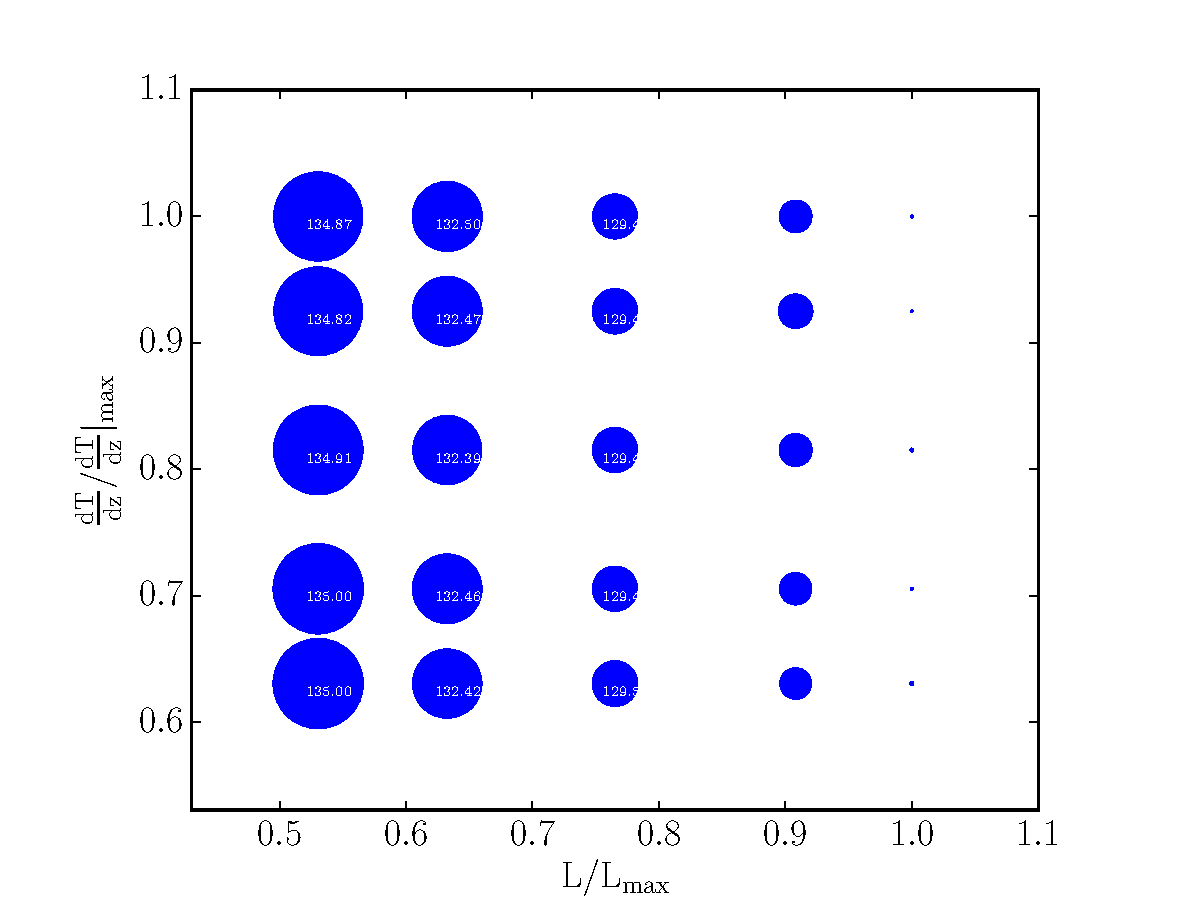
\includegraphics[width=0.60\textwidth]{realz_quad300K}
  &
  \hspace{-9mm}
  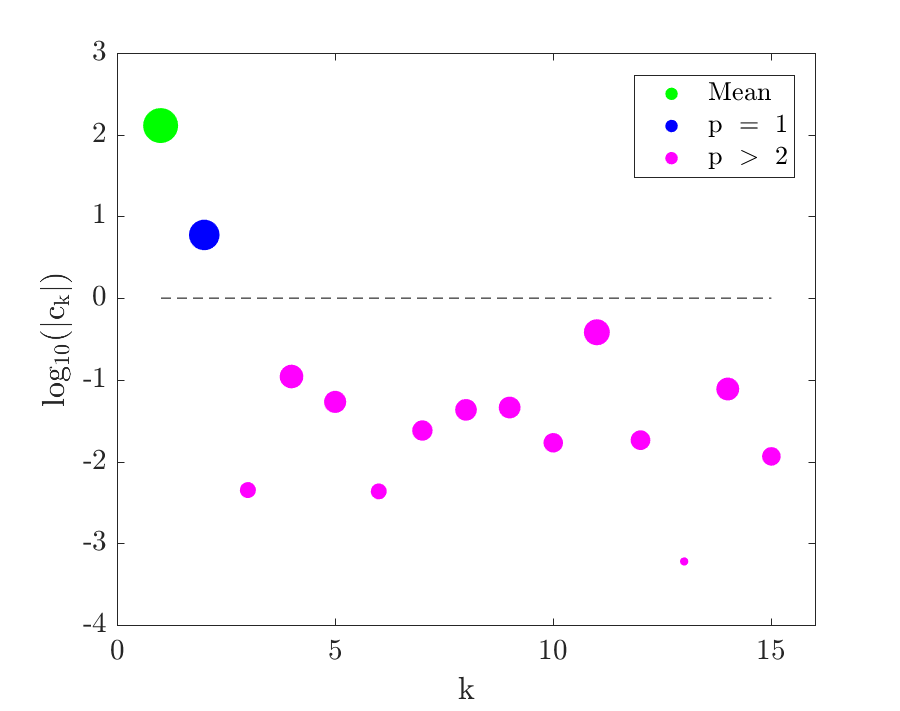
\includegraphics[width=0.56\textwidth]{PCspectrum_300}
  \\ (a) & (b)
  \end{tabular}
\caption{(a) Realizations of discrepancy in bulk thermal conductivity at the Gauss-Legendre quadrature notes are
depicted using circles. The size of the circle in each case is proportional to the discrepancy estimate, also provided
 in cases where it is observed to be relatively large. (b) Spectrum of PC coefficients is depicted using circles of
 varying sizes, proportional to the log value of their magnitude. The above computations were performed at 300 K.}
\label{fig:rs1}
\end{center}
\end{figure}

\begin{figure}[htbp]
\begin{center}
\begin{tabular}{cc}
 \hspace{-10mm}
  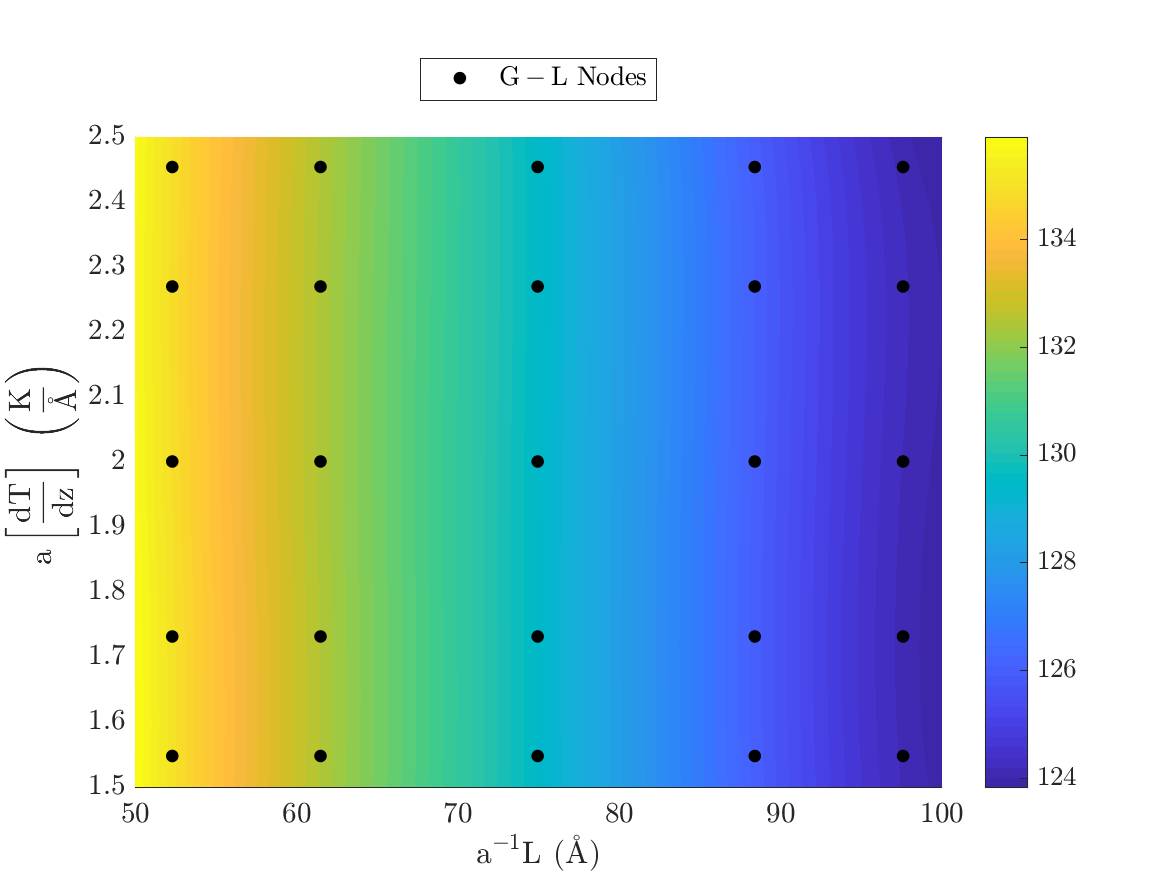
\includegraphics[width=0.55\textwidth]{err2D_300}
  &
  %\hspace{-9mm}
  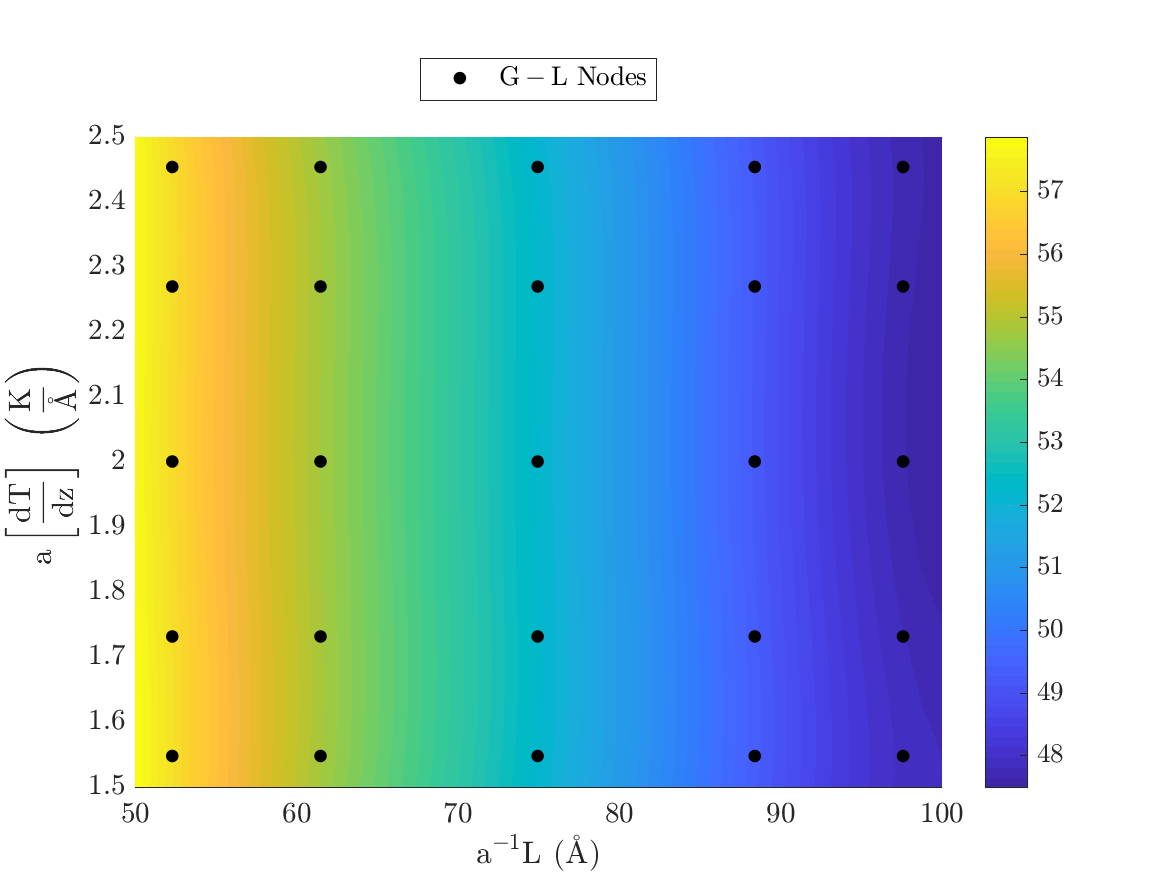
\includegraphics[width=0.55\textwidth]{err2D_500}
  \\ (a) & (b)
  \end{tabular}
  \\ \vspace{1mm}
  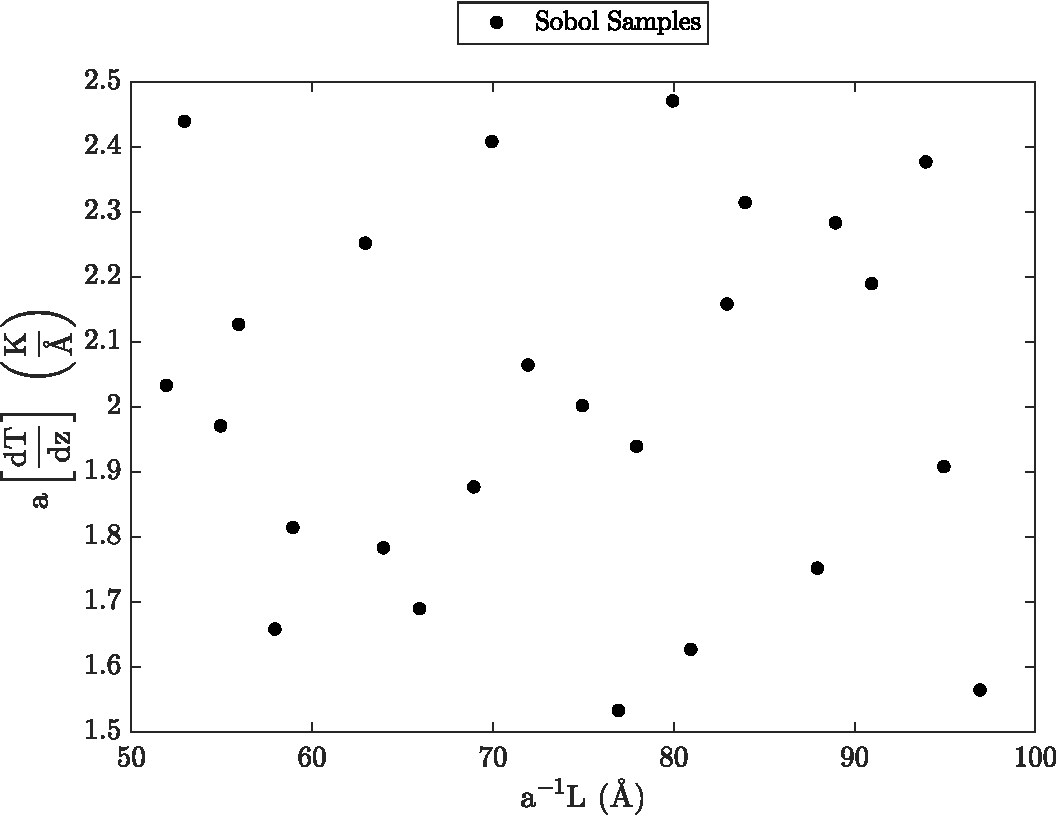
\includegraphics[width=0.50\textwidth]{err2D_s}
  \\ (c)
\caption{Response surface of the discrepancy in bulk thermal conductivity at (a) $T$ = 300~K and
 (b) $T$ = 500~K. Gauss-Legendre quadrature nodes are highlighted in both cases. (c) Sobol samples
 in the 2D domain used for verifying the accuracy of the response surfaces. Here, $|a|$ denotes the magnitude
 of the lattice constant.}
\label{fig:rs2}
\end{center}
\end{figure}

As expected, the discrepancy is observed to decrease
 with the bar length ($L$) due to increase in the mean free path. It is however interesting to note that the 
 variation in discrepancy due to changes in the applied temperature gradient in the considered range is found to be
 negligible. The accuracy of the response surface is verified by computing a relative L-2 norm of the error
 ($\varepsilon_{\tiny{\mbox{L-2}}}$) on an independent set of Sobol samples~\cite{Saltelli:2010}
(see Figure~\ref{fig:rs2}(c)) in the 2D 
 parameter domain as follows:
 
 \be
 \varepsilon_{\tiny{\mbox{L-2}}} = \frac{\left[\sum_{j}(\epsilon_{\tiny{\mbox{d},j}}^{\mbox{\tiny{MD}}} - 
 \epsilon_{\tiny{\mbox{d},j}}^{\mbox{\tiny{PCE}}})^2\right]^{\frac{1}{2}}}{\left[\sum_j(\epsilon_{\tiny{\mbox{d},j}}
 ^{\mbox{\tiny{MD}}})^2\right]^{\frac{1}{2}}} 
 \label{eq:err_l2}
 \ee
 
 A response surface was also constructed at $T$ = 1000~K (plot not included for brevity) and the impact of
 varying the temperature gradient on the discrepancy was still observed to be negligible. In all cases,
 $\varepsilon_{\tiny{\mbox{L-2}}}$ in Eq.~\ref{eq:err_l2} was estimated to be of $\mathcal{O}(10^{-3})$ thereby
 indicating that the response surfaces could be used to predict the discrepancy for a given
 point ($L$,$\frac{dT}{dz}$) in the considered domain with reasonable accuracy. As an additional verification
 step, we plot the inverse of thermal conductivity against the inverse of bar length using data from NEMD
 simulations as well as predictions from the response surface 
($\kappa_{\mbox{\tiny{MD}}}~=~\kappa_{\mbox{\tiny{E}}}~-~\epsilon_{\mbox{\tiny{d}}}$) in Figure~\ref{fig:kinv}.
%
\begin{figure}[htbp]
\begin{center}
\begin{tabular}{cc}
 \hspace{-10mm}
  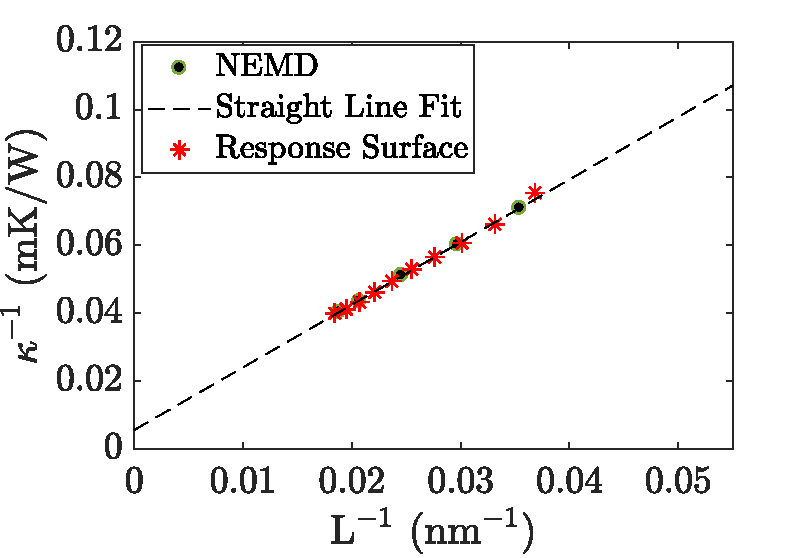
\includegraphics[width=0.50\textwidth]{kinv_300}
  &
  %\hspace{-9mm}
  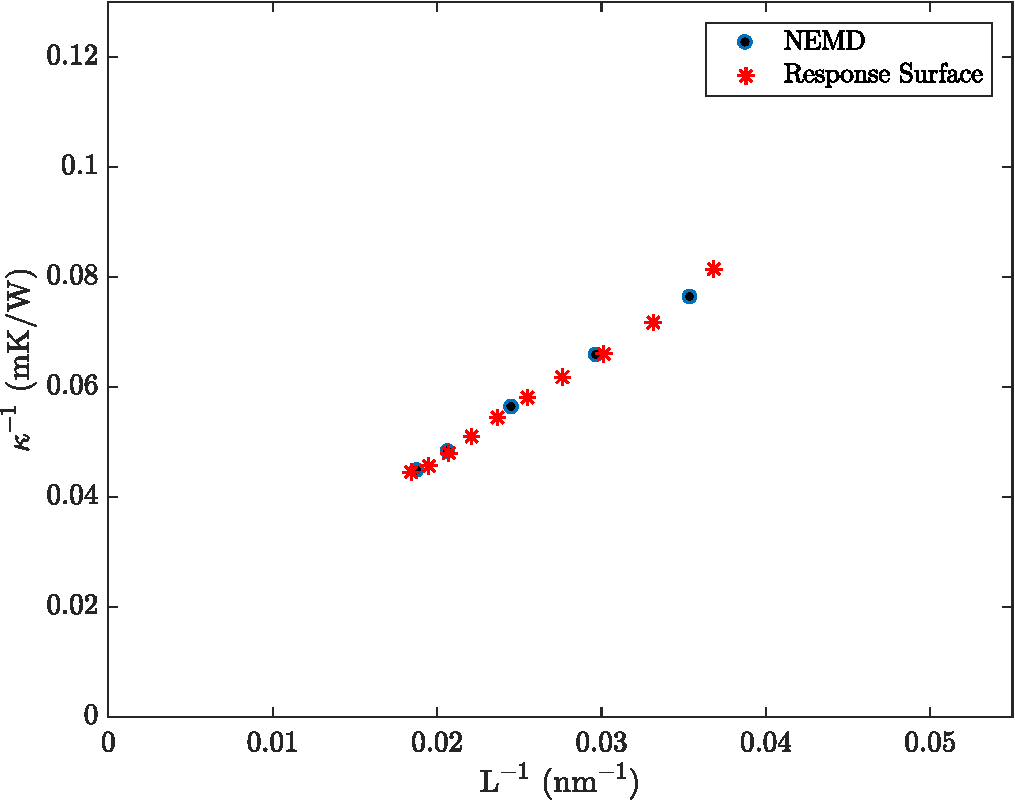
\includegraphics[width=0.50\textwidth]{kinv_500}
  \\ (a) & (b)
  \end{tabular}
 \caption{Inverse of the bulk thermal conductivity estimates are plotted against the inverse of Si bar length
 using predictions from NEMD as well as estimates from the response surface at (a)  $T$ = 300~K and 
 (b) $T$ = 500~K. A straight line fit to the estimates is also illustrated in each case.}
\label{fig:kinv}
\end{center}
\end{figure}
%
It is observed that the response surface estimates exhibit an expected linear trend, consistent with NEMD
  predictions. Using the y-intercept of the straight line fit, the bulk thermal conductivity was estimated
 as 178.52 W/m/K and 110.64 W/m/K at 300~K and 500~K respectively. Using a wider range for system length would
help improve these estimates. However, as discussed earlier, our focus is on demonstrating
a methodology for quantifying the uncertainties (with limited resources) in bulk thermal conductivity predictions
 using NEMD as opposed
to determining accurate estimates for the same. Constructing response surfaces using a
 relatively small number of NEMD predictions thus offers
  potential for huge computational savings for studies aimed at predicting thermal conductivity trends and 
  quantifying the discrepancy with measurements for a wide range of system sizes, applied temperature gradients as 
  well as bulk temperatures.

In the following sections, we shift our focus towards understanding the impact of the uncertainty
in SW potential parameter values on the uncertainty in NEMD predictions for bulk
thermal conductivity in Si.  
 




































